\chapter{Einleitung}

Im Rahmen verschiedener E-Learning-Szenarien gibt es die 
Problematik, dass ein Lerner etwas modellieren soll. Das 
Modell des Lerners muss dann auf seine Korrektheit 
überprüft werden. Bei der Modellierung soll dem Lerner 
zusätzlich ein hilfreiches Feedback gegeben werden.

Ein Beispiel dafür ist das Programm \emph{ChemNom}. Dabei 
soll der Lerner Moleküle verschiedener Stoffe zeichnen.
\emph{ChemNom} unterstützt den Lerner, indem es beispielsweise 
Aussagen über noch fehlende Atome oder ungültige Bindungen 
macht.

\begin{figure}[htb]
	\centering
		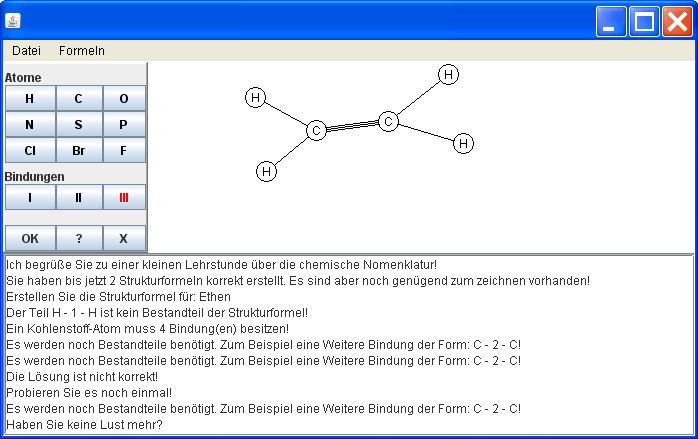
\includegraphics[width=0.7\linewidth,keepaspectratio]{bilder/chemnom.png}
	\caption{Das Programm \emph{ChemNom}}
	\label{fig:chemnom}
\end{figure}

Für diese Arbeit wird davon ausgegangen, dass die 
Modelle als Graphen vorliegen, da sich mit Graphen sehr 
viele Modelle darstellen lassen. 
Im Fall von \emph{ChemNom} würden die Moleküle als Graphen dargestellt, 
indem man die Atome als Knoten interpretiert und die Bindungen 
als Kanten.

Des Weiteren ist eine Musterlösung gegeben. Die Eingabe des 
Lerners soll dann mit der Musterlösung verglichen werden. 
Dabei stellt sich die Frage nach der Machbarkeit einer 
solchen Überprüfung.

\section{Korrektheit und Fehlergröße}
Die erste Frage, die sich stellt, ist: Wann ist eine 
eingegebene Lösung korrekt? Da eine Musterlösung vorliegt, 
wird eine Lösung als korrekt definiert, wenn sie mit der 
Musterlösung identisch ist. Falls es mehrere richtige Lösungen 
gibt, kann man mehrere Musterlösungen angeben.

Bei einem Lernprozess ist es jedoch vermutlich 
häufiger der Fall, dass die vorgeschlagene Lösung nicht 
korrekt ist. Um dem Lerner ein Feedback geben zu können, 
ist es somit nötig zusätzliche Aussagen über eine falsche 
Lösung zu treffen. Ein erster Ansatz ist dabei ein Maß, 
um zwischen verschiedenen Graden an fehlerhaften Lösungen 
zu unterscheiden. In dieser Arbeit sei dieses Maß der 
Aufwand, der nötig ist, um die Lösung des Lerners in die 
Musterlösung umzuwandeln. Dieser Aufwand wird als 
Graphabstand bezeichnet.

Um zu überprüfen, ob eine Lösung (des Lerners) korrekt ist 
oder um eine Aussage über die Fehler in einer Lösung zu 
treffen, ist es notwendig Knoten und Kanten der Lösung den 
entsprechenden Knoten und Kanten in der Musterlösung 
zuzuordnen. Dies ist nicht trivial. In \cite{Bravo:2006} 
wird das Problem damit umgangen, dass die Bezeichnung der 
Knoten in der Eingabe des Lerners mit Namenslisten abgeglichen 
wird, oder der Lerner selbst die Zuordnung vornimmt.

\section{Ziele und Anforderungen}
Ziel dieser Arbeit ist die Schaffung einer algorithmischen 
Grundlage, um in einer Modellierungsaufgabe den Lösungsvorschlag 
eines Lerners zu überprüfen und zu bewerten. Dabei soll die 
Zuordnung der Knoten zueinander automatisch erfolgen.

Für ein Verfahren zur Auswertung einer Lösung stellen sich 
dabei einige Anforderungen. Das Verfahren sollte möglichst 
unabhängig vom konkreten Modell arbeiten. Zusätzlich ist 
eine geringe Laufzeit wünschenswert. Im Idealfall bekommt 
der Lerner ohne spürbare Verzögerung eine Rückmeldung 
zu seiner Eingabe. Auch wenn die Berechnung länger dauert, 
sollte sie nicht mehr als ein paar Sekunden benötigen.

\section{Vorhaben}
Um die genannten Ziele zu erreichen, befasst sich diese Arbeit 
zuerst mit einigen Grundlagen im Bereich der Graphentheorie. 
Danach sollen verschiedene algorithmische Ansätze vorgestellt 
und untersucht werden. Fällt die Untersuchung positiv aus, dann 
wird zusätzlich ein Konzept vorgestellt, mit dem sich weitere 
Aussagen über die Eingabe eines Lerners treffen lassen.
